%
%Не забыть:
%--------------------------------------
%Вставить колонтитулы, поменять название на титульнике



%--------------------------------------

\documentclass[a4paper, 12pt]{article} 

%--------------------------------------
%Russian-specific packages
%--------------------------------------
%\usepackage[warn]{mathtext}
\usepackage[T2A]{fontenc}
\usepackage[utf8]{inputenc}
\usepackage[english,russian]{babel}
\usepackage[intlimits]{amsmath}
\usepackage{esint}
%--------------------------------------
%Hyphenation rules
%--------------------------------------
\usepackage{hyphenat}
\hyphenation{ма-те-ма-ти-ка вос-ста-нав-ли-вать}
%--------------------------------------
%Packages
%--------------------------------------
\usepackage{amsmath}
\usepackage{amssymb}
\usepackage{amsfonts}
\usepackage{amsthm}
\usepackage{latexsym}
\usepackage{mathtools}
\usepackage{etoolbox}%Булевые операторы
\usepackage{extsizes}%Выставление произвольного шрифта в \documentclass
\usepackage{geometry}%Разметка листа
\usepackage{indentfirst}
\usepackage{wrapfig}%Создание обтекаемых текстом объектов
\usepackage{fancyhdr}%Создание колонтитулов
\usepackage{setspace}%Настройка интерлиньяжа
\usepackage{lastpage}%Вывод номера последней страницы в документе, \lastpage
\usepackage{soul}%Изменение параметров начертания
\usepackage{hyperref}%Две строчки с настройкой гиперссылок внутри получаеммого
\usepackage[usenames,dvipsnames,svgnames,table,rgb]{xcolor}% pdf-документа
\usepackage{multicol}%Позволяет писать текст в несколько колонок
\usepackage{cite}%Работа с библиографией
\usepackage{subfigure}% Человеческая вставка нескольких картинок
\usepackage{tikz}%Рисование рисунков
\usepackage{float}% Возможность ставить H в положениях картинки
% Для картинок Моти
\usepackage{misccorr}
\usepackage{lscape}
\usepackage{cmap}

% Для Х И М И И

\usepackage[version=4]{mhchem}



\usepackage{graphicx,xcolor}
\graphicspath{{Pictures/}}
\DeclareGraphicsExtensions{.pdf,.png,.jpg}

%----------------------------------------
%Список окружений
%----------------------------------------
\newenvironment {theor}[2]
{\smallskip \par \textbf{#1.} \textit{#2}  \par $\blacktriangleleft$}
{\flushright{$\blacktriangleright$} \medskip \par} %лемма/теорема с доказательством
\newenvironment {proofn}
{\par $\blacktriangleleft$}
{$\blacktriangleright$ \par} %доказательство
%----------------------------------------
%Список команд
%----------------------------------------
\newcommand{\grad}
{\mathop{\mathrm{grad}}\nolimits\,} %градиент

\newcommand{\diver}
{\mathop{\mathrm{div}}\nolimits\,} %дивергенция

\newcommand{\rot}
{\ensuremath{\mathrm{rot}}\,}

\newcommand{\Def}[1]
{\underline{\textbf{#1}}} %определение

\newcommand{\RN}[1]
{\MakeUppercase{\romannumeral #1}} %римские цифры

\newcommand {\theornp}[2]
{\textbf{#1.} \textit{ #2} \par} %Написание леммы/теоремы без доказательства

\newcommand{\qrq}
{\ensuremath{\quad \Rightarrow \quad}} %Человеческий знак следствия

\newcommand{\qlrq}
{\ensuremath{\quad \Leftrightarrow \quad}} %Человеческий знак равносильности

\renewcommand{\phi}{\varphi} %Нормальный знак фи

\newcommand{\me}
{\ensuremath{\mathbb{E}}}

\newcommand{\md}
{\ensuremath{\mathbb{D}}}



%\renewcommand{\vec}{\overline}




%----------------------------------------
%Разметка листа
%----------------------------------------
\geometry{top = 3cm}
\geometry{bottom = 2cm}
\geometry{left = 1.5cm}
\geometry{right = 1.5cm}
%----------------------------------------
%Колонтитулы
%----------------------------------------
\pagestyle{fancy}%Создание колонтитулов
\fancyhead{}
%\fancyfoot{}
%----------------------------------------
%Интерлиньяж (расстояния между строчками)
%----------------------------------------
%\onehalfspacing -- интерлиньяж 1.5
%\doublespacing -- интерлиньяж 2
%----------------------------------------
%Настройка гиперссылок
%----------------------------------------
\hypersetup{				% Гиперссылки
	unicode=true,           % русские буквы в раздела PDF
	pdftitle={Заголовок},   % Заголовок
	pdfauthor={Автор},      % Автор
	pdfsubject={Тема},      % Тема
	pdfcreator={Создатель}, % Создатель
	pdfproducer={Производитель}, % Производитель
	pdfkeywords={keyword1} {key2} {key3}, % Ключевые слова
	colorlinks=true,       	% false: ссылки в рамках; true: цветные ссылки
	linkcolor=blue,          % внутренние ссылки
	citecolor=blue,        % на библиографию
	filecolor=magenta,      % на файлы
	urlcolor=cyan           % на URL
}
%----------------------------------------
%Работа с библиографией (как бич)
%----------------------------------------
\renewcommand{\refname}{Список литературы}%Изменение названия списка литературы для article
%\renewcommand{\bibname}{Список литературы}%Изменение названия списка литературы для book и report
%----------------------------------------
\begin{document}
	\begin{titlepage}
		\begin{center}
			$$$$
			$$$$
			$$$$
			$$$$
			{\Large{НАЦИОНАЛЬНЫЙ ИССЛЕДОВАТЕЛЬСКИЙ УНИВЕРСИТЕТ}}\\
			\vspace{0.1cm}
			{\Large{ВЫСШАЯ ШКОЛА ЭКОНОМИКИ}}\\
			\vspace{0.25cm}
			{\large{Факультет физики}}\\
			\vspace{5.5cm}
			{\Huge\textbf{{Экзамен}}}\\%Общее название
			\vspace{1cm}
			{\LARGE{<<Химия>>}}\\%Точное название
			\vfill
			
\includegraphics[width = 0.2\textwidth]{HSElogo}\\
			\vfill
			Москва\\
			2020
		\end{center}
	\end{titlepage}

\tableofcontents

\newpage

\section{Вещество. Классификация химических веществ. Химические элементы. Атом, атомный номер, относительная атомная масса, изотопы.}

\textbf{Вещество} --- нечто, состоящее из атомов; нечто, в чем выделение атомов невозможно или теряет физический смысл (например, плазма или звёздное вещество), к предмету рассмотрения химией не относят.

Согласно химической классификации, химические вещества делятся на индивидуальные (чистые) вещества и смеси.

В свою очередь, чистые вещества делятся на простые (состоящие из атомов одного элемента) и сложные. Простые в свою же очередь делятся по своим свойствам на металлы (имеют характерный блеск, высокую теплопроводность и электропроводность, обычно твердые и т.п.) и неметаллы (не обладают блеском, ковкостью, обычно газ и т.п.). Сложные же делятся на органические (соединения углерода) и неорганические (все остальные).

Смеси же делятся на растворы (однородная система с потенциально непостоянным составом, это их отличие от химического соединения) и механические смеси (неоднородные, взвеси).

\textbf{Атом} --- частица вещества микроскопических размеров и массы, наименьшая часть химического элемента, являющаяся носителем его свойств.

\textbf{Атомный номер} (зарядовое число) --- количество протонов в атомном ядре. Равно заряду ядра в единицах элементарного заряда и является порядковым номером соответствующего химического элемента в таблице Менделеева.

Атомная масса измеряется в \textbf{относительных атомных единицах} (а. е. м./углеродная единица) --- единицах массы, определяемых как 1/12 массы свободного покоящегося атома углерода \ce{^12 C}.

\begin{equation}
	1 \text{ а. е. м} = 1.660 539 066 60(5) \cdot 10^{-27} \text{ кг}
\end{equation}

\textbf{Изотопы} --- разновидность атомов одного и того же химического вещества (т.е. атомы имеют одинаковое число протонов), сходные по свойствам (а именно по структуре электронных оболочек), но отличающиеся массой ядер. Изотопы также иногда называются нуклидами. Различие по массе происходит из-за различного числа нейтронов в ядрах.

Масса, которая указывается в таблице Менделеева, является средневзвешенной по распространенности в природе массой изотопов вещества.




\newpage

\section{Периодическая система химических элементов. Структура таблицы Д.И. Менделеева, группы, периоды и блоки. Металлы и неметаллы.}

\Def{Периодический закон}

Свойства химических элементов, а также формы и свойства образуемых ими простых веществ и соединений, находятся в периодической зависимости от величины зарядов ядер их атомов.

\subsection{Периодическая таблица}

\begin{figure}[H]
    \centering
    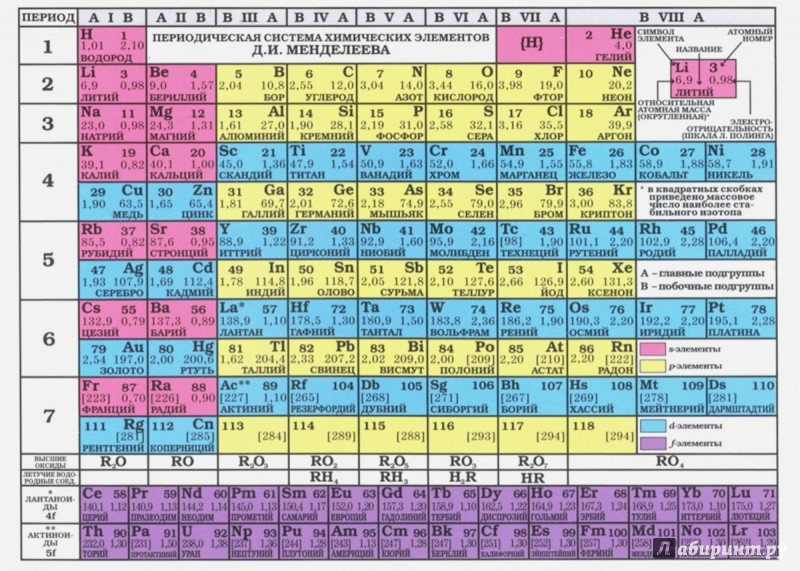
\includegraphics[width = \textwidth]{TeX/Pictures/2_table.jpg}
    \caption{Периодическая таблица Менделеева: краткая форма}
    \label{fig:table}
\end{figure}

\subsection{Структура}
\Def{Период}

Ряд в таблице Менделеева; последовательность элементов, начинающаяся щелочным металлом (или водородом) и заканчивающаяся инертным газом. 

В направлении «слева направо» атомный радиус обычно сокращается (в силу того, что у каждого последующего элемента увеличивается количество заряженных частиц, и электроны притягиваются ближе к ядру), и параллельно с ним возрастает энергия ионизации и электроотрицательность.

\Def{Группа}

Столбец в таблице Менделеева. 

Высшая степень окисления равна номеру группы со знаком «плюс». Низшая определяется, как номер группы минус 8.

Элементы одной группы проявляют схожие свойства, поэтому группы часто имеют особые названия:

\begin{table}[H]
    \centering
    \begin{tabular}{c|c}
    \hline
        Номер группы (подгруппы) &  Название\\
         1 (кроме H) &  Щелочные металлы \\
         2 (кроме Mg, Be) &  Щелочноземельные металлы \\
         16 &  Халькогены \\
         17 &  Галогены \\
         18 &  Инертные газы \\
    \hline
    \end{tabular}
    \caption{Названия некоторых групп периодической системы}
    \label{tab:groups}
\end{table}

 По направлению сверху вниз в рамках группы радиус атома возрастает (чем больше у него заполненных энергетических уровней, тем дальше от ядра располагаются валентные электроны), а энергия ионизации и электроотрицательность снижается (связи в атоме ослабевают, и, следовательно, изъять электрон становится проще).
 
 \Def{Блоки}
 
 Деление в соответствии с оболочкой, на которой находится последний электрон.
 
 \begin{figure}[H]
     \centering
     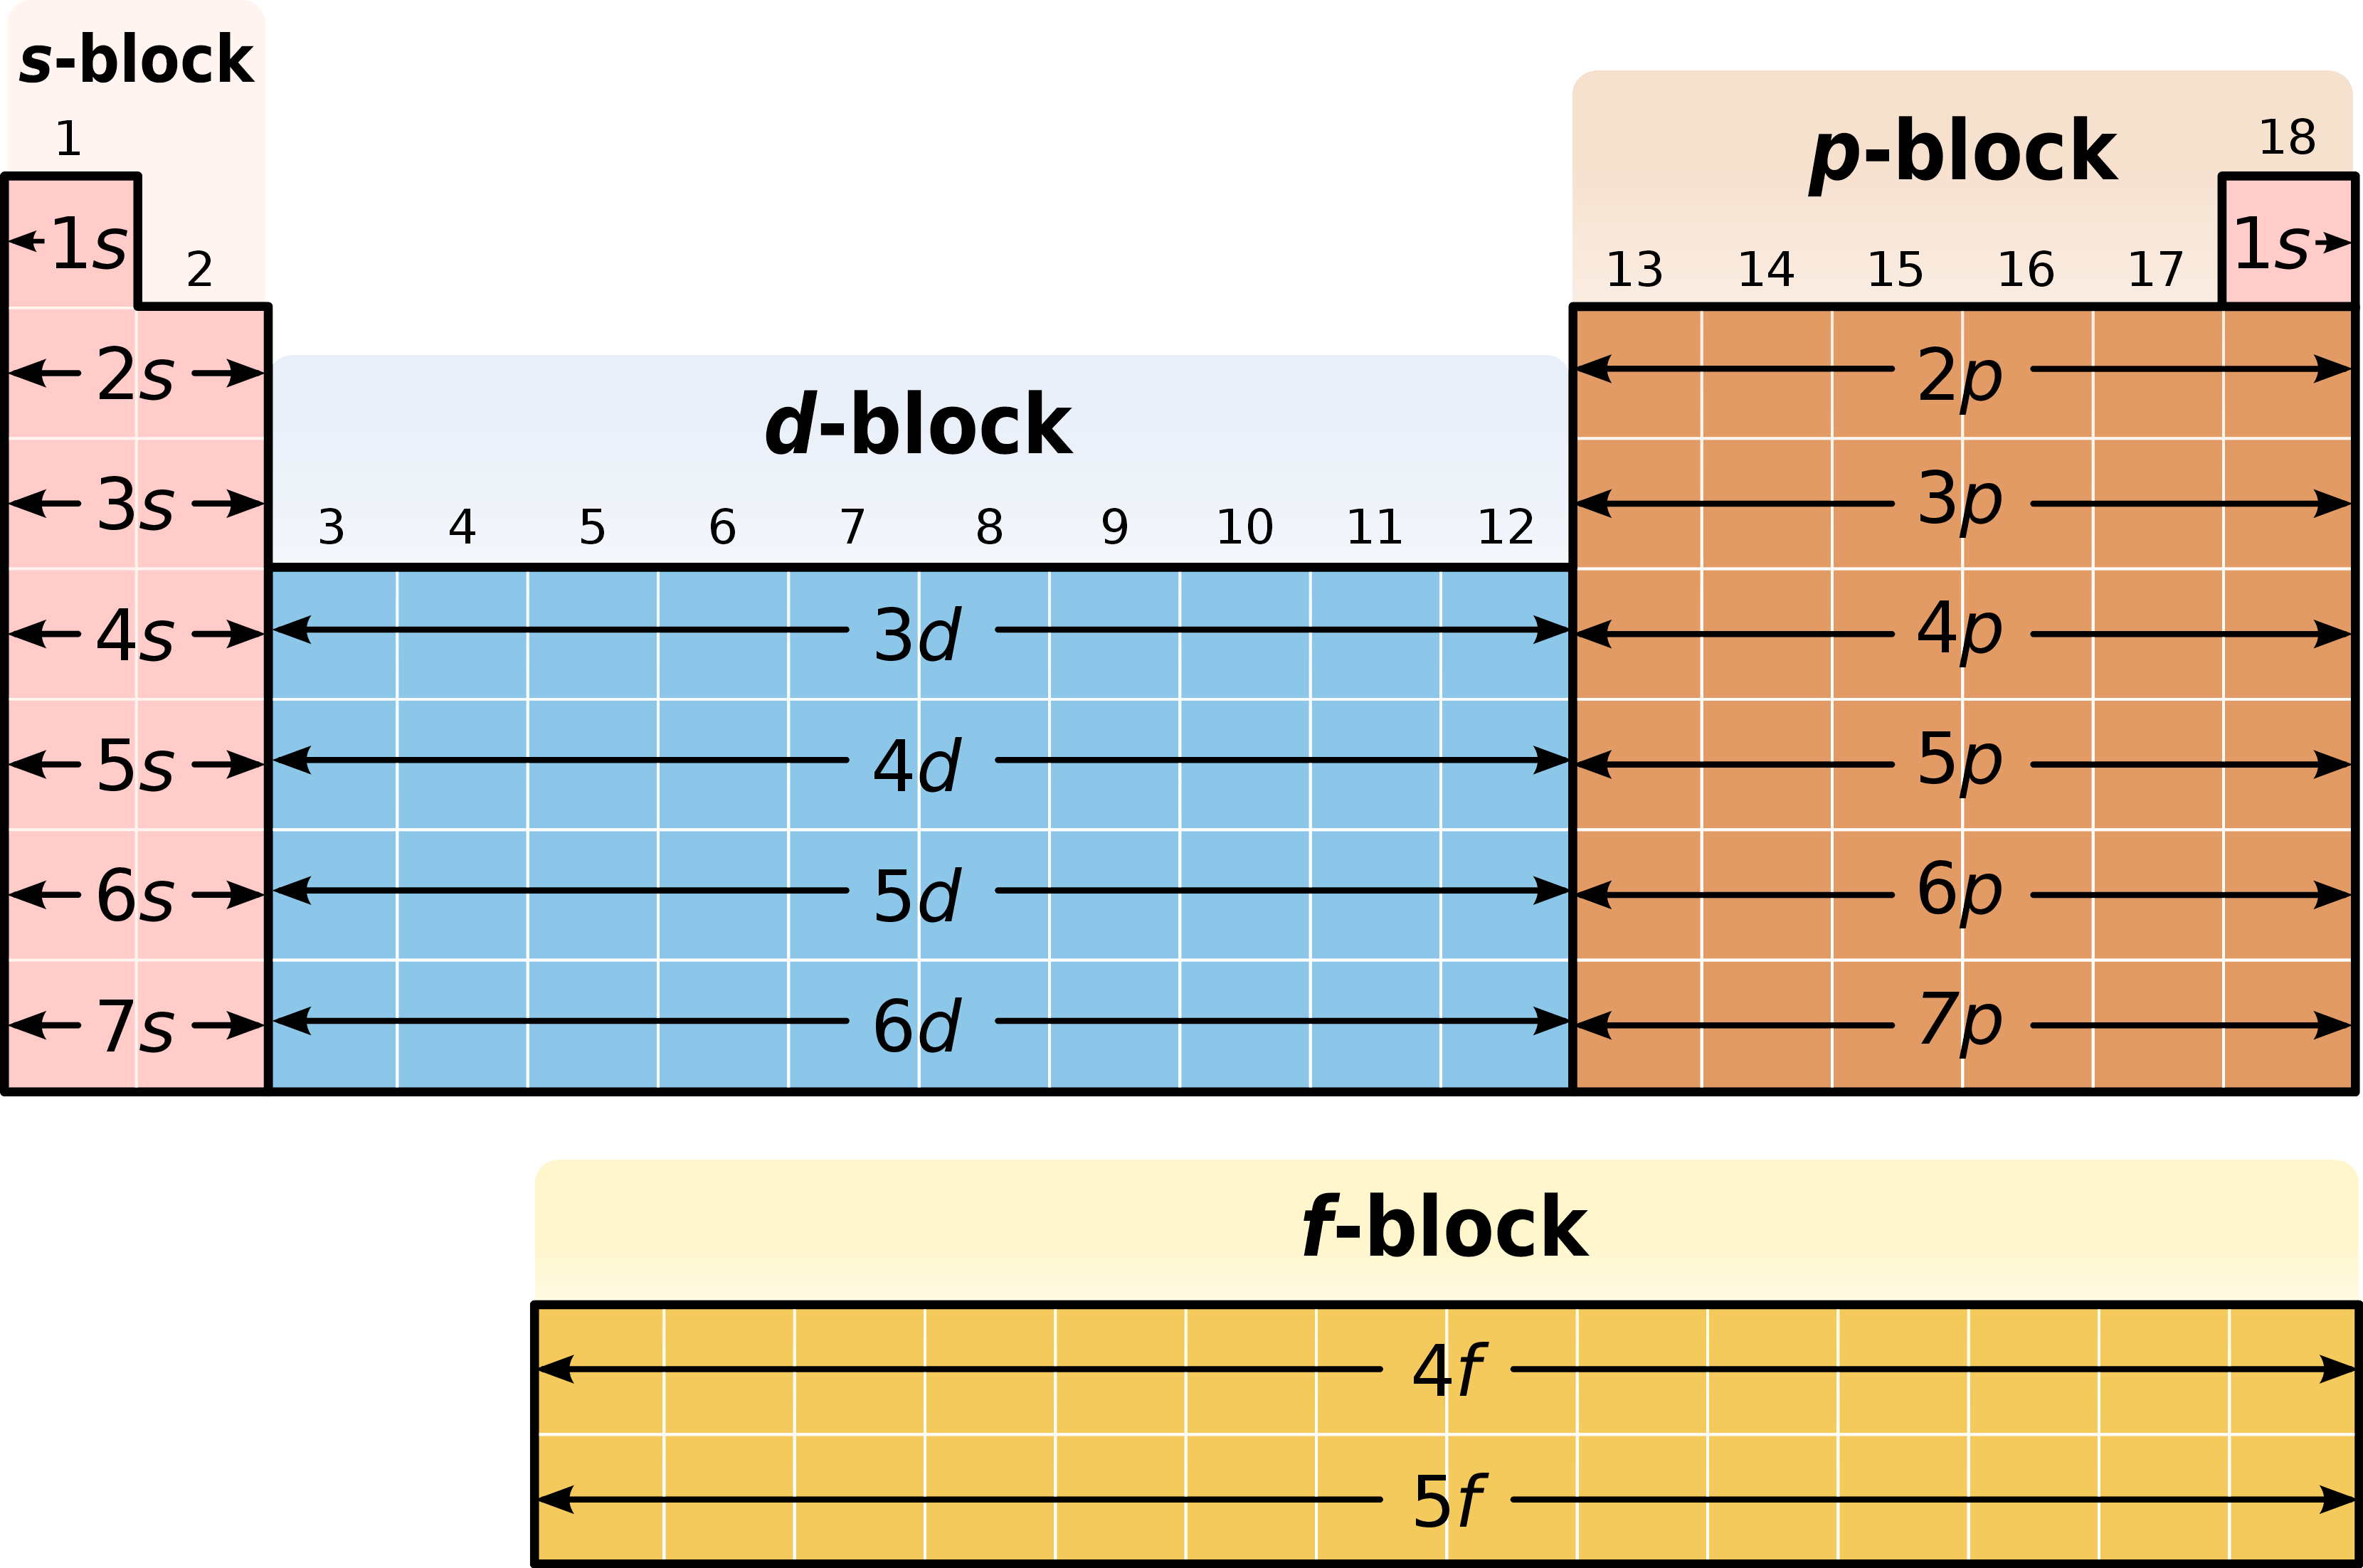
\includegraphics[width = \textwidth]{TeX/Pictures/2_block.png}
     \caption{Деление на блоки}
     \label{fig:block}
 \end{figure}
 
 \subsection{Металлы и неметаллы}
 
Традиционно деление на 2 группы: металлы имеют высокую тепло- и электропроводность, положительный температурный коэффициент сопротивления, высокую пластичность, ковкость и металлический блеск; неметаллы же определяют большая способность к присоединению дополнительных электронов, и проявление более высокой окислительной активности, чем у металлов.

\begin{figure}[H]
    \centering
    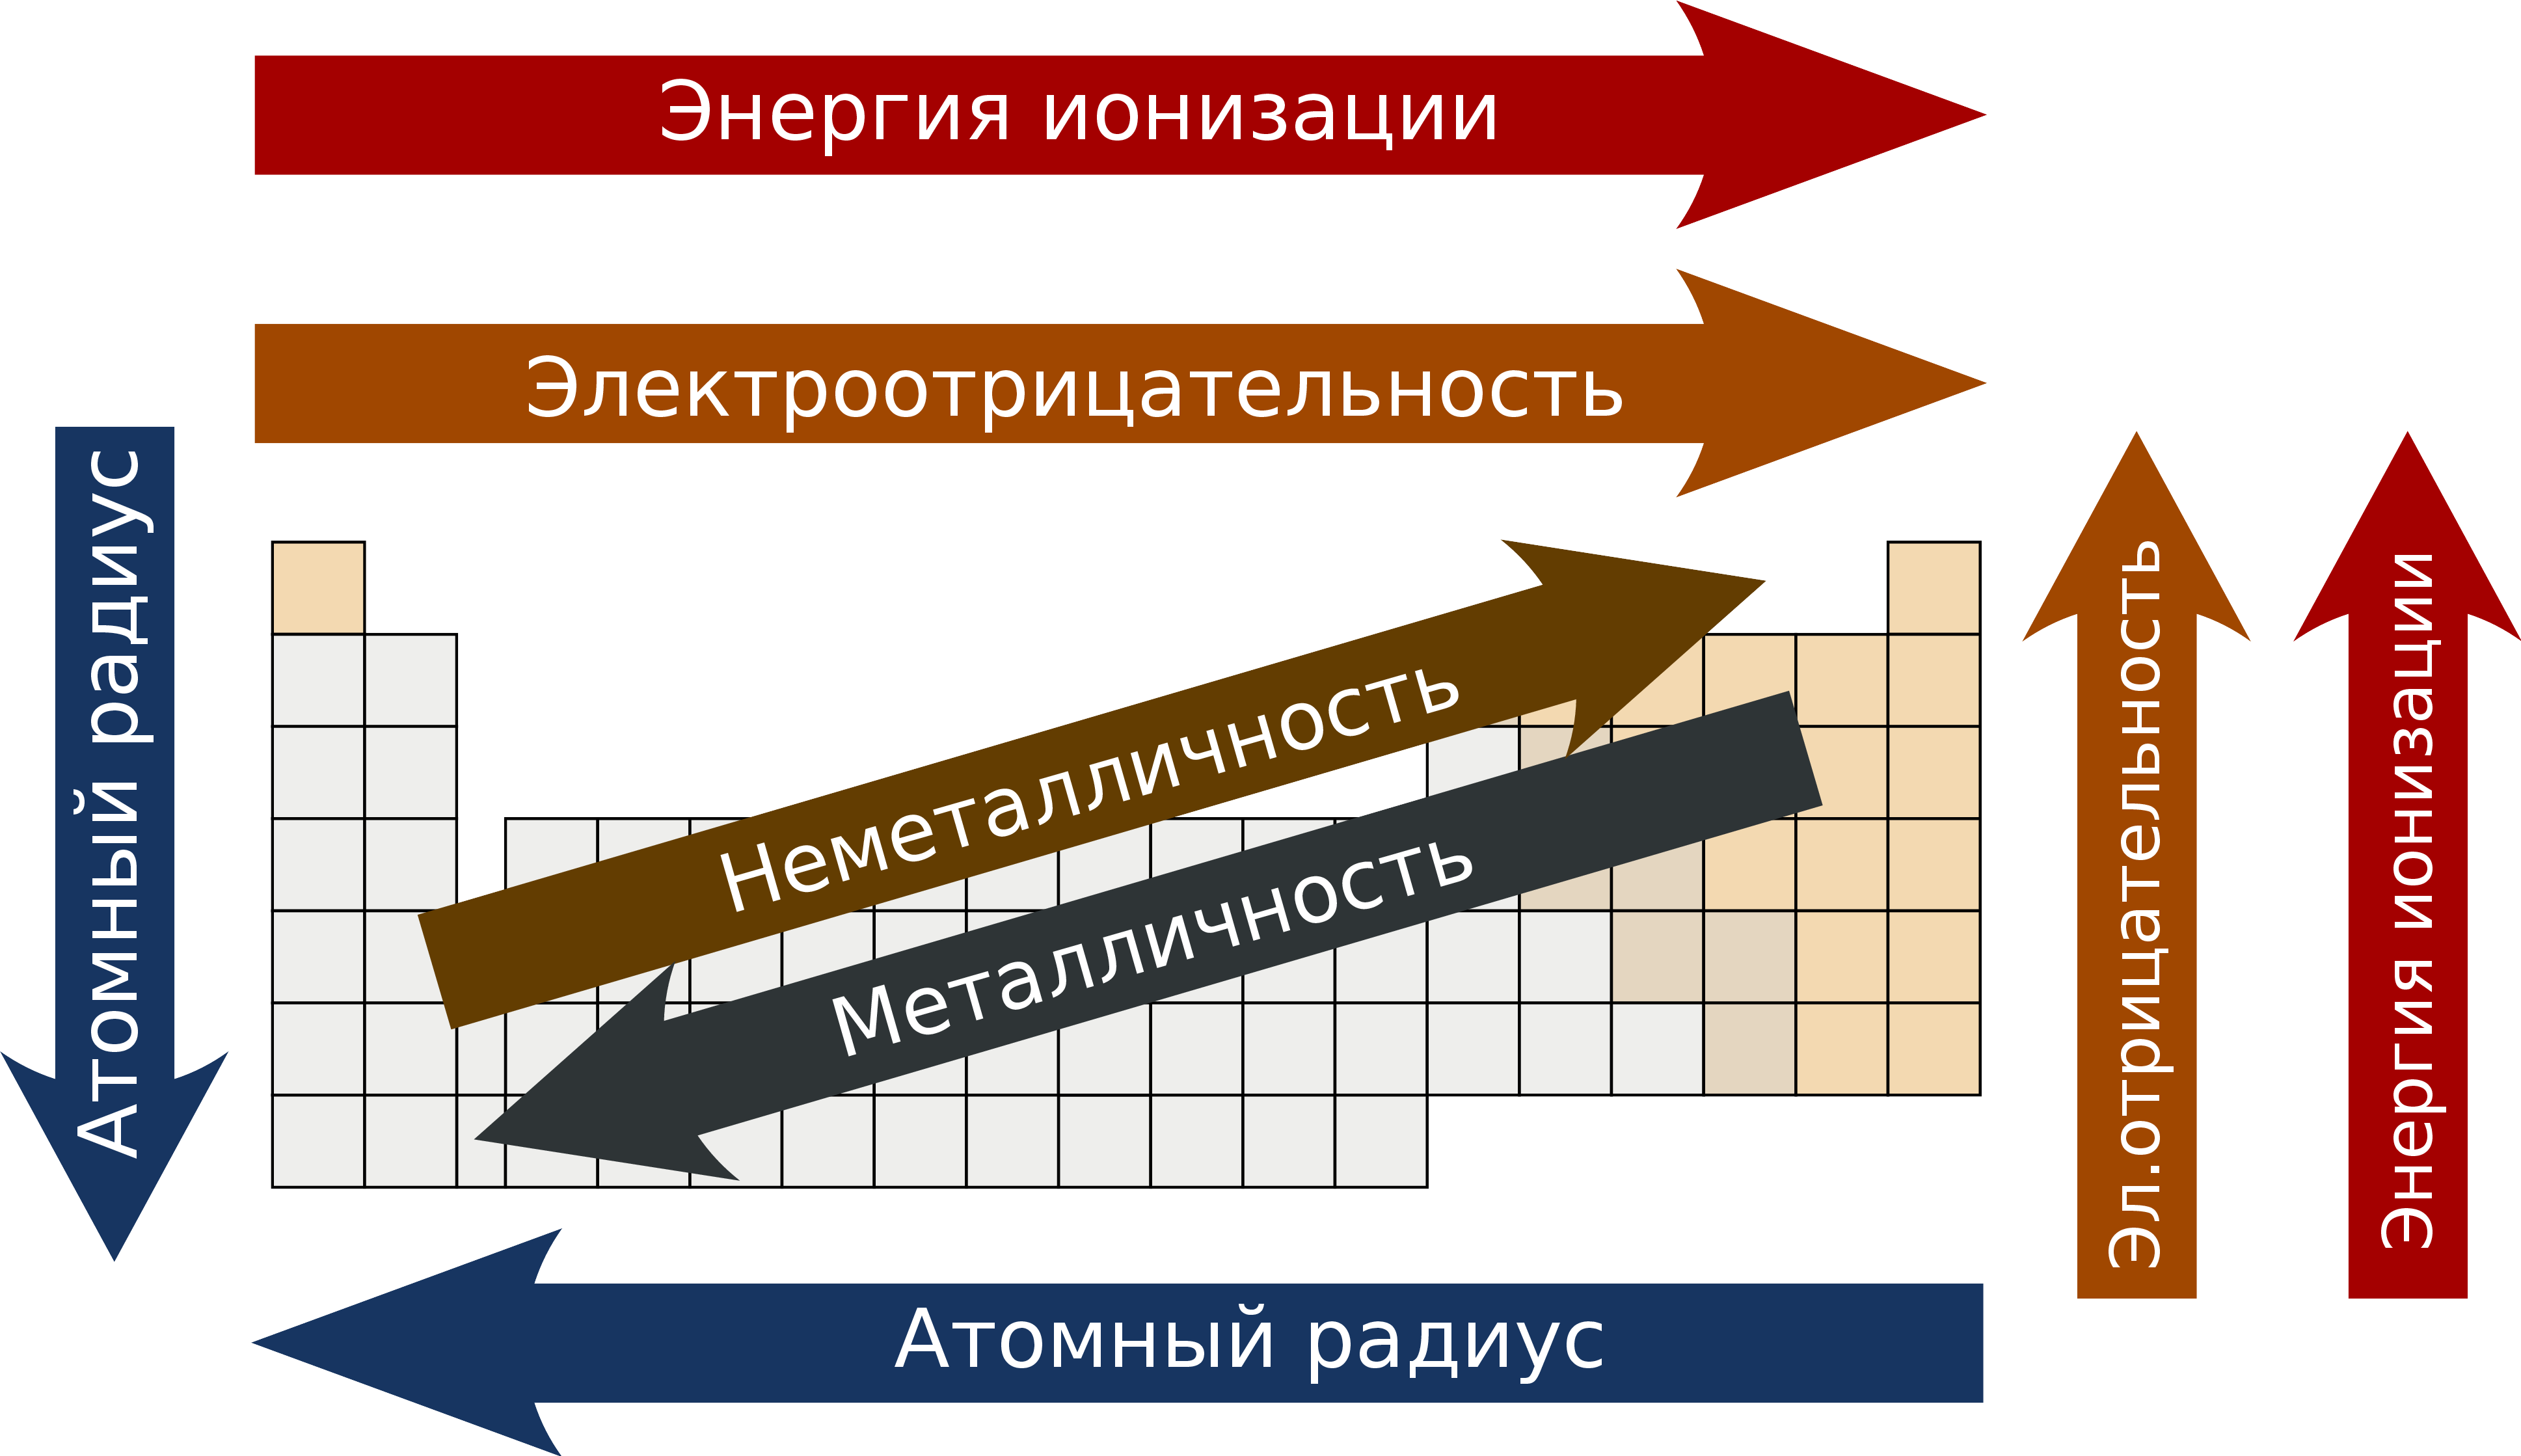
\includegraphics[width = \textwidth]{TeX/Pictures/2_properties.png}
    \caption{Свойства элементов}
    \label{fig:properties}
\end{figure}

Металлы, взаимодействуя с неметаллами, чаще образуют ионные соединения:

\ce{2 Na + Cl_2 = 2 NaCl}

Металлы, взаимодействуя друг с другом, образуют сплавы, обладающими всеми свойствами чистых металлов.

Неметаллы, взаимодействуя друг с другом, часто образуют летучие соединения с молекулярной связью:

\ce{2P+3Cl_2=2PCl_3}



\newpage

\section{Химические соединения и их характеристики: строение, состав, свойство. Простые и сложные соединения. Стехиометрические соотношения, эмпирическая и молекулярная формула соединения. Валентность элементов.}

\textbf{Химическое соединение} --- сложное вещество, состоящее из химически связанных атомов одного или более элементов. \\ 

\textbf{Простыми} называются вещества, состоящие из атомов одного химического элемента. Например, молекулярные кислород \ce{O2}, водород \ce{H2} и т.д. \textit{Атомарные газы} (типа гелия \ce{He}, аргона \ce{Ar}) назвать \textit{соединениями} нельзя.\\

\textbf{Состав} соединения записывается в виде химической формулы: 

\begin{itemize}
	\item \textit{эмпирическая (простейшая) формула} описывает только соотношение количества элементов в молекуле. Для бензола, например, это \ce{CH}.
	\item \textit{молекулярная формула} отражает число атомов в молекуле. Для бензола \ce{C6H6}. 
\end{itemize}

\textbf{Структурная формула} показывает взаимное расположение атомов в молекуле.

\begin{figure}[H]
	\centering
	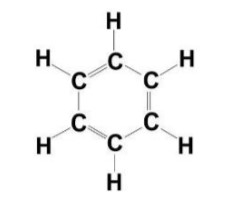
\includegraphics{Pictures/Benzol.jpg}
	\caption{Структурная формула бензола.}
\end{figure}

Соединения характеризуются \textbf{химическими свойствами}: 
\begin{itemize}
	\item способностями реагировать с другими веществами; 
	\item способностью к разложению (реакции, в которой из одного, более
сложного вещества образуется 2 и более других, более простых);
	\item диссоциации (процессу распада на ионы при растворении в воде или плавлении вещества).\\
\end{itemize}

\textit{Молекула} --- электронейтральная частица, состоящая из двух или более атомов.\\

\textbf{Валентность} --- число химических связей, которыми данный атом в молекуле связан с другими. \textit{Для веществ ионного строения:} валентность --- максимальное число одновалентных атомов (например, водорода), которые могут соединяться с атомом данного элемента или на которые этот атом может замещаться.

Валентность обозначается римскими цифрами и может принимать значения от одного до восьми. 

\begin{figure}[H]
	\centering
	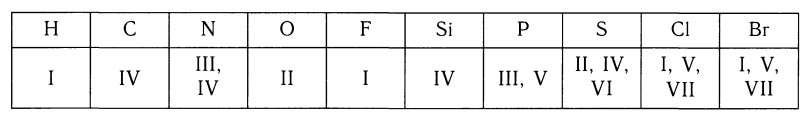
\includegraphics{Pictures/Val.jpg}
	\caption{Характерные валентности некоторых элементов-неметаллов.}
\end{figure}

\textbf{Стехиометрия} --- раздел химии, посвященный расчетам по химическим формулам и уравнениям реакций.\\

\textbf{Основной закон химической стехиометрии:}

\emph{Отношение количеств реагирующих веществ (в молях) равно отношению соответствующих коэффициентов в уравнении реакции.}\\

Например, для реакции \ce{2H2 + O2 -> 2H2O} количества прореагировавших веществ относятся как:

\begin{equation*}
n(\ce{H2}): n(\ce{O2}): n(\ce{H2O}) = 1:2:1.
\end{equation*}


\newpage

\section{}

\newpage

\section{}

\newpage

\section{Квантовые числа электрона. Принципы заполнения орбиталей. Электронная формула атома и иона. Диаграмма энергетических уровней атома.}

\subsection{Квантовые числа}
Состояние электрона в атоме описывают с помощью четырех квантовых чисел: главного (n), орбитального (l), магнитного (m) и спинового (s).

 

\Def{Главное квантовое число}

Определяет энергетический уровень электрона, принимает целые значения $(n = 1, 2, 3 ...)$. Номер периода атома = число энергетических уровней атома.

Например:

Элемент кадмий Cd расположен в пятом периоде, значит $n = 5$. В его атоме электроны раcпределены по пяти энергетическим уровням $(n = 1, n = 2, n = 3, n = 4, n = 5)$; внешним будет пятый уровень $(n = 5)$. 

\Def{Орбитальное квантовое число}

 Характеризует геометрическую форму орбитали. Принимает значение целых чисел от 0 до (n - 1). Набор орбиталей с одинаковыми значениями n называется энергетическим уровнем, c одинаковыми n и l - подуровнем. Обозначаются буквами s,p,d,f...
 
 \Def{Магнитное квантовое число} 
 
 Принимает целочисленные значения от -l до +l. 
 
 \subsection{Принципы заполнения орбиталей}
 
\Def{Принцип Паули}
 
 В атоме может быть двух электронов, у которых значения всех квантовых чисел (n, l, m, s) были бы одинаковы, т.е. на каждой орбитали может находиться не более двух электронов (c противоположными спинами).
 
 \Def{Правило Клечковского (принцип наименьшей энергии)}:
 
 Заполнение электронами орбиталей в атоме происходит в порядке возрастания суммы главного и орбитального квантовых чисел n + l. При одинаковой сумме раньше заполняется орбиталь с меньшим значением n.

1s < 2s < 2p < 3s < 3p < 4s < 3d < 4p < 5s < 4d < 5p < 6s < 5d < 4f < 6p < 7s

 \Def{Правила Хунда}
 
 \begin{itemize}
     \item Минимальной энергией обладает терм с максимальным значением S
     \item Из термов с одинаковым значением S наименьшей энергией обладает терм с максимальным значением L
 \end{itemize}
 
 \subsection{Электронная формула атома и иона}
 
 Максимальное число электронов на энергетическом уровне равно $2n^2$ (n - номер энергетического уровня).
 
 Энергетический уровень может быть завершенным или незавершенным. В завершенном энергетическом уровне все орбитали заполнены, электроны спарены.

Заполнение энергетических уровней идет по принципу наименьшей энергии. Электрон занимает орбиталь с наименьшей энергией.

\begin{figure}[H]
    \centering
    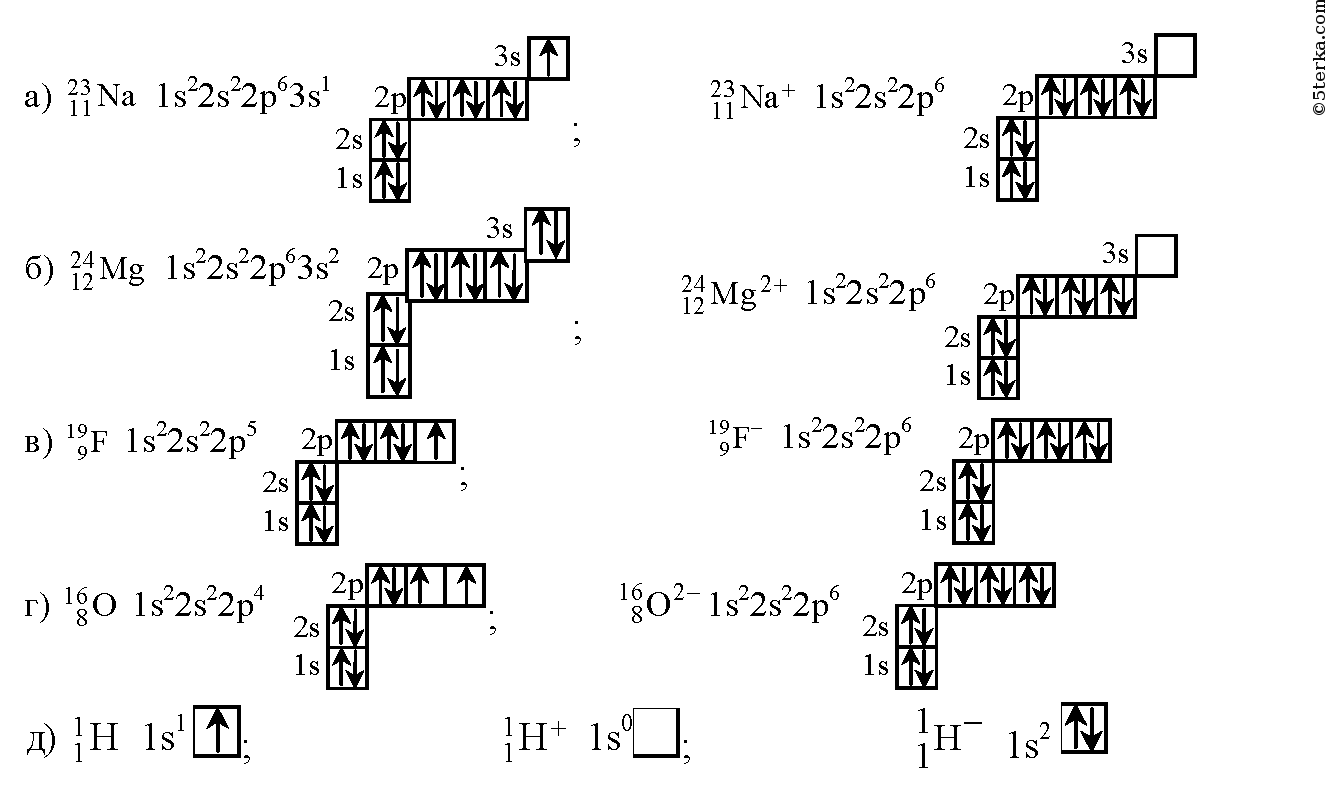
\includegraphics[width = \textwidth]{Pictures/6_atom.png}
    \caption{Примеры формул электронного строения и диаграмм уровней}
    \label{fig:7atom}
\end{figure}



\newpage

\section{Квантовые числа электрона. Принципы заполнения орбиталей. Электронная формула атома и иона. Диаграмма энергетических уровней атома.}

\subsection{Квантовые числа}
Состояние электрона в атоме описывают с помощью четырех квантовых чисел: главного (n), орбитального (l), магнитного (m) и спинового (s).

 

\Def{Главное квантовое число}

Определяет энергетический уровень электрона, принимает целые значения $(n = 1, 2, 3 ...)$. Номер периода атома = число энергетических уровней атома.

Наример,

Элемент кадмий Cd расположен в пятом периоде, значит $n = 5$. В его атоме электроны раcпределены по пяти энергетическим уровням $(n = 1, n = 2, n = 3, n = 4, n = 5)$; внешним будет пятый уровень $(n = 5)$. 

\Def{Орбитальное квантовое число}

 Характеризует геометрическую форму орбитали. Принимает значение целых чисел от 0 до (n - 1). Набор орбиталей с одинаковыми значениями n называется энергетическим уровнем, c одинаковыми n и l - подуровнем. Обозначаются буквами s,p,d,f...
 
 \Def{Магнитное квантовое число} 
 
 Принимает целочисленные значения от -l до +l. 
 
 \subsection{Принципы заполнения орбиталей}
 
\Def{Принцип Паули}
 
 В атоме может быть двух электронов, у которых значения всех квантовых чисел (n, l, m, s) были бы одинаковы, т.е. на каждой орбитали может находиться не более двух электронов (c противоположными спинами).
 
 \Def{Правило Клечковского (принцип наименьшей энергии).}
 
 Заполнение электронами орбиталей в атоме происходит в порядке возрастания суммы главного и орбитального квантовых чисел n + l. При одинаковой сумме раньше заполняется орбиталь с меньшим значением n.

1s < 2s < 2p < 3s < 3p < 4s < 3d < 4p < 5s < 4d < 5p < 6s < 5d < 4f < 6p < 7s

 \Def{Правила Хунда}
 
 \begin{itemize}
     \item Минимальной энергией обладает терм с максимальным значением S
     \item Из термов с одинаковым значением S наименьшей энергией обладает терм с максимальным значением L
 \end{itemize}
 
 \subsection{Электронная формула атома и иона}
 
 Максимальное число электронов на энергетическом уровне равно $2n^2$ (n - номер энергетического уровня).
 
 Энергетический уровень может быть завершенным или незавершенным. В завершенном энергетическом уровне все орбитали заполнены, электроны спарены.

Заполнение энергетических уровней идет по принципу наименьшей энергии. Электрон занимает орбиталь с наименьшей энергией.

\begin{figure}[H]
    \centering
    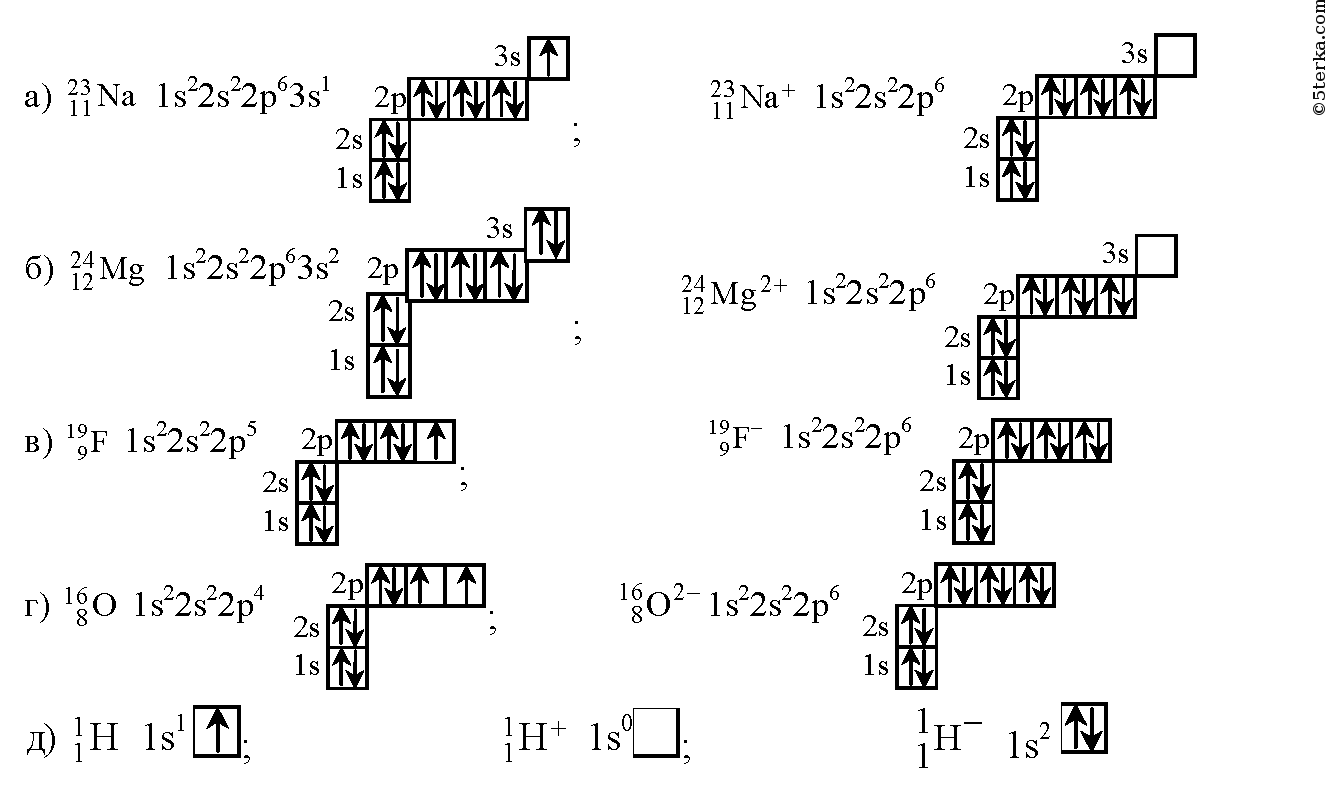
\includegraphics[width = \textwidth]{/7_atom.png}
    \caption{Примеры формул электронного строения и диаграмм уровней}
    \label{fig:7atom}
\end{figure}



\newpage

\section{}

\newpage

\section{Классификация химических реакций. Стехиометрическое описание химической реакции. Энергетическая кривая элементарной химической реакции. Прямая и обратная реакции.}
\subsection{Химические реакции и их классификации}
\textbf{Химическая реакция}  -- превращение одного или нескольких исходных веществ (\textbf{реагентов}) в другие вещества (\textbf{продукты}), при котором ядра атомов не меняются, при этом происходит перераспределение электронов и ядер, и образуются новые химические вещества.

Классификацию химических реакций можно проводить по разным параметрам. Далее приведено несколько варииантов.
\begin{itemize}
    \item По типу превращений реагирующих частиц: 
    \begin{enumerate}
        \item \textbf{Реакция соединения} -- химическая реакция, в результате которой из двух или большего числа исходных веществ образуется только одно новое. В такие реакции могут вступать как простые, так и сложные вещества. Примером может служить окисление лития с получением оксида лития:
        \begin{equation*}
            \ce{4Li + O2 -> 2Li2O}
        \end{equation*}
        \item \textbf{Реакция разложения} -- химическая реакция, в результате которой из одного вещества образуется несколько новых веществ. В реакции данного типа вступают только сложные соединения, а их продуктами могут быть как сложные, так и простые вещества. Примером может служить разложение угольной кислоты на воду и углекислый газ:
        \begin{equation*}
            \ce{H2CO3 -> H2O + CO2 ^}
        \end{equation*}
        \item \textbf{Реакция замещения} -- химическая реакция, в результате которой атомы одного элемента, входящие в состав простого вещества, замещают атомы другого элемента в его сложном соединении. Как следует из определения, в таких реакциях одно из исходных веществ должно быть простым, а другое сложным. Примером может послужить реакция лития (простое вещество) с водой (сложное), с получением гидроксида лития (сложное вещество) и водорода (простое):
        \begin{equation*}
            \ce{2Li + 2H2O -> 2LiOH + H2 ^}
        \end{equation*}
        \item \textbf{Реакции обмена} — реакция, в результате которой два сложных вещества обмениваются своими составными частями. Примером может послужить рассмотренная ранее реакция нейтрализации соляной кислоты и гидроксида натрия с получением поваренной соли и воды:
\begin{equation}
    \ce{HCl + NaOH -> NaCl + H2O}
\end{equation}
    \end{enumerate}
    \item По направлению протекания:
    \begin{enumerate}
        \item \textbf{Необратимые} химические реакции, <<протекающие лишь в одном направлении>>  в том смысле, что реагенты реагируют с получением продуктов, но продукты реакции не реагируют с получением реагентов.  О таких химических процессах говорят, что они протекают «до конца». К ним относят реакции горения, а также реакции, сопровождающиеся образованием малорастворимых или газообразных веществ. Примером может послужить горение углерода (с получением углекислого газа):
        \begin{equation*}
            \ce{C + O2 -> CO2 ^}
        \end{equation*}
        \item \textbf{Обратимыми} называются химические реакции, <<протекающие одновременно в двух противоположных направлениях>>. В уравнениях таких реакций знак равенства заменяется двумя противоположно направленными стрелками. Среди двух одновременно протекающих реакций различают прямую (протекает «слева направо») и обратную (протекает «справа налево»). Поскольку в ходе обратимой реакции исходные вещества одновременно и расходуются, и образуются, они не полностью превращаются в продукты реакции. Поэтому об обратимых реакциях говорят, что они протекают «не до конца». В результате всегда образуется смесь исходных веществ и продуктов взаимодействия. Примером может послужить гидролиз (то есть реакция с водой) нитрита натрия:
        \begin{equation*}
            \ce{NaNO2 + H2O <--> HNO2 + NaOH}
        \end{equation*}
    \end{enumerate}
    \item По тепловому эффекту:
    \begin{enumerate}
        \item \textbf{Экзотермические реакции} -- реакции, которые идут с выделением тепла, (положительный тепловой эффект) например, реакции горения. Так же показательным примером являются реакции активных металлов с водой, далее дана такая реакция для натрия:
        \begin{equation*}
            \ce{2Na + 2H2O -> 2NaOH + H_{2} ^} + Q
        \end{equation*}
        $Q$ -- выделевшееся тепло.
        \item \textbf{Эндотермические реакции} в ходе которых тепло поглощается (отрицательный тепловой эффект) из окружающей среды. Характерный пример разложение карбоната кальция на оксид кальция и углекислый газ при нагреве:
        \begin{equation*}
            \ce{CaCO3 ->[t^{\circ}] CaO + CO2 ^}
        \end{equation*}
        \end{enumerate}
\end{itemize}
Так же реакции можно классифицировать по агрегатному состоянию реагентов и продуктов, по наличию каталлизатора или ингибитора или самопроизвольности (по изменению энергии Гиббса). Выделяют важнейший класс реакций, в которых атомы одного элемента (\textbf{окислителя}) восстанавливаются, то есть присоединяют электроны и понижают свою степень окисления, а атомы другого элемента (\textbf{восстановителя}) окисляются, то есть отдают электроны и повышают свою степень окисления. Такие реакции называются \textbf{окислительно-восстановительными} (сокращённо ОВР).
\subsection{Стехиометрическое описание химической реакции.}
Стехиометрия -- система законов, правил и терминов, обосновывающих расчёты состава веществ и количественных [относительных] соотношений между массами (объёмами для газов) веществ в химических реакциях. Стехиометрия включает нахождение химических формул, составление уравнений химических реакций, расчёты, применяемые в препаративной химии и химическом анализе.

Для большинства реакций можно записать химическое уравнение, в правой части которого стоят реагенты, а в левой -- продукты (вместо знака равно между ними обычно пишут значок \ce{->}). Большинство уравнений реакций написанных в этом конспекте используют стехиометрические правила.  Стехиометрическое уравнение — уравнение, показывающее количественные соотношения реагентов и продуктов химической реакции. Общий вид стехиометрического уравнения химической реакции таков:

\begin{equation}
    \sum_{i = 1}^{N}n_{i}X_{i} = \sum_{j = 1}^{M}m_{j}Y_{i}, \ \text{где} \ N,M,n_{i},m_{i}\in\mathbb{N}
\end{equation}
Натуральные числа $n_{i}$ и $m_{j}$ называются стехиометрическими коэффициентами. Эта запись означает, что  $n_{1}$ молекул реагента $X_{1}$, $n_{2}$ молекул реагента $X_{2}$, …, $n_{N}$ молекул реагента $X_{N}$, вступив в реакцию, образуют $m_{1}$ молекул вещества $Y_{1}$, $m_2$ молекул вещества $Y_{2}$, …,  $m_{M}$ молекул вещества $Y_{M}$. 

Коэффициенты $n_{i}$ и $m_{j}$ определяются так, чтобы количества атомов одного и того же вещества и справа и слева оставалось одним и тем же (тем самым удовлетворяется \textit{химичность} реакции (т.к. элементы не изменяются), а так же выполняется закон сохранения массы). Расчёт коэффициентов $n_{i}$ и $m_{j}$ для данных реагентов и продуктов называется уравниванием коэффициентов, и может производиться разными методами, например подбором с учётом валентностей, однако реакции с несколькими сложными реагентами и продуктами уравнять таким образом довольно сложно, поэтому используются другие методы (например электронный баланс в случае ОВР).
\subsection{Энергетическая кривая химической реакции. }
\begin{figure}[H]
\centering
\begin{tikzpicture}[>=latex']
    \draw[domain=-3:3.5, samples=100, red, thick] plot (\x,{(1/2 + abs(\x)/(2*\x))*(3*exp(- \x*\x)) + (1/2 - abs(\x)/(2*\x))*(1 + 2*exp(- \x*\x))});
    \draw[dashed] (-3.5,1) -- (0.5,1);
    \draw[dashed] (3.5,0) -- (-0.5,0);
    \draw[dashed] (-3.5,3) -- (2.75,3);
    \draw[<->,blue] (0,0) -- (0,1) node[left, pos=0.5, black] {$\Delta H$};
    \draw[->] (-3,-0.8) -- (-3,3.4) node[above]{$E$};
    \draw[->] (-3.5,-0.5) -- (3.7,-0.5) node[right]{$\xi$};
    \draw[<->,blue] (-2.5,1) -- (-2.5,3) node[right, pos=0.5, black]{$\Delta E_{\longrightarrow}$};
    \draw[<->,blue] (2.5,0) -- (2.5,3) node[right, pos=0.5, black]{$\Delta E_{\longleftarrow}$};
\end{tikzpicture}
\caption{Энергетическая кривая. $E_{\longrightarrow}$ -- энергия активации прямой реакции, $E_{\longleftarrow}$ -- энергия активации обратной реакции.}
\label{fig:energycurve}
\end{figure}
Точное определение химической переменной $\xi_{i}$ может быть задано так:
\begin{equation}
    \xi_{i} = \frac{\mathrm{d}\mathcal{V}_{i}}{\mathrm{d}n_{i}} = \frac{\Delta \mathcal{V}_{i}}{\Delta n_{i}} = \pm\frac{\Delta \mathcal{V}_{i}}{n_{i}}
\end{equation}
Здесь $\mathcal{V}_{i}$ -- количество молей $i$-того реагента (для продукта координата определяется так же только с минусом), а $n_{i}$ -- его стехиометрический коэффициент в уравнении рассматриваемой реакции. Изменение $\Delta$ подразумевает разницу между началом реакции и каким-то моментом её протекания. Так как $n_{i}$ входит только  в одну из сторон уравнения, то $\Delta n_{i} = \pm n_{i} $, где плюс выбирается для реагента, а минус для продукта реакции.

Для химической реакции или процесса энергетическая кривая  является теоретическим представлением единственного энергетического пути вдоль координаты реакции, когда реагенты превращаются в продукты. Диаграммы координат реакций выводятся из соответствующей поверхности потенциальной энергии (ППЭ) (так как таких обобщённых координат у любой кривой вообще говоря несколько), которые используются в вычислительной химии для моделирования химических реакций, связывая энергию молекулы (молекул) с ее структурой (в рамках приближения Борна – Оппенгеймера ). Координата реакции - это параметрическая кривая, которая следует за ходом реакции и показывает ее ход.

На рисунке~\ref{fig:energycurve} привидён пример энергетической кривой элементарной реакции\footnote{Элементарна реакция в том смысле, что у графика один пик, соответствующий прямому переходу из реагента в продукт. Большее количество пиков соответствовало бы нескольким промежуточным продуктам.}. Так как $\Delta E_{\longrightarrow} < \Delta E_{\longleftarrow}$ прямая реакция является экзотермической, а обратная -- эндотермическая, при этом высвобождаемая или сообщаемая теплота равна $\Delta H$. Внесение катализатора соответствовало бы снижению горба кривой, а ингибитора наоборот -- завышению, то есть высота горба характерезует скорость протечения реакции.


\newpage

%
%Не забыть:
%--------------------------------------
%Вставить колонтитулы, поменять название на титульнике



%--------------------------------------

\documentclass[a4paper, 12pt]{article} 

%--------------------------------------
%Russian-specific packages
%--------------------------------------
%\usepackage[warn]{mathtext}
\usepackage[T2A]{fontenc}
\usepackage[utf8]{inputenc}
\usepackage[english,russian]{babel}
\usepackage[intlimits]{amsmath}
\usepackage{esint}
%--------------------------------------
%Hyphenation rules
%--------------------------------------
\usepackage{hyphenat}
\hyphenation{ма-те-ма-ти-ка вос-ста-нав-ли-вать}
%--------------------------------------
%Packages
%--------------------------------------
\usepackage{amsmath}
\usepackage{amssymb}
\usepackage{amsfonts}
\usepackage{amsthm}
\usepackage{latexsym}
\usepackage{mathtools}
\usepackage{etoolbox}%Булевые операторы
\usepackage{extsizes}%Выставление произвольного шрифта в \documentclass
\usepackage{geometry}%Разметка листа
\usepackage{indentfirst}
\usepackage{wrapfig}%Создание обтекаемых текстом объектов
\usepackage{fancyhdr}%Создание колонтитулов
\usepackage{setspace}%Настройка интерлиньяжа
\usepackage{lastpage}%Вывод номера последней страницы в документе, \lastpage
\usepackage{soul}%Изменение параметров начертания
\usepackage{hyperref}%Две строчки с настройкой гиперссылок внутри получаеммого
\usepackage[usenames,dvipsnames,svgnames,table,rgb]{xcolor}% pdf-документа
\usepackage{multicol}%Позволяет писать текст в несколько колонок
\usepackage{cite}%Работа с библиографией
\usepackage{subfigure}% Человеческая вставка нескольких картинок
\usepackage{tikz}%Рисование рисунков
\usepackage{float}% Возможность ставить H в положениях картинки
% Для картинок Моти
\usepackage{misccorr}
\usepackage{lscape}
\usepackage{cmap}

% Для Х И М И И

\usepackage{mhchem}



\usepackage{graphicx,xcolor}
\graphicspath{{Pictures/}}
\DeclareGraphicsExtensions{.pdf,.png,.jpg}

%----------------------------------------
%Список окружений
%----------------------------------------
\newenvironment {theor}[2]
{\smallskip \par \textbf{#1.} \textit{#2}  \par $\blacktriangleleft$}
{\flushright{$\blacktriangleright$} \medskip \par} %лемма/теорема с доказательством
\newenvironment {proofn}
{\par $\blacktriangleleft$}
{$\blacktriangleright$ \par} %доказательство
%----------------------------------------
%Список команд
%----------------------------------------
\newcommand{\grad}
{\mathop{\mathrm{grad}}\nolimits\,} %градиент

\newcommand{\diver}
{\mathop{\mathrm{div}}\nolimits\,} %дивергенция

\newcommand{\rot}
{\ensuremath{\mathrm{rot}}\,}

\newcommand{\Def}[1]
{\underline{\textbf{#1}}} %определение

\newcommand{\RN}[1]
{\MakeUppercase{\romannumeral #1}} %римские цифры

\newcommand {\theornp}[2]
{\textbf{#1.} \textit{ #2} \par} %Написание леммы/теоремы без доказательства

\newcommand{\qrq}
{\ensuremath{\quad \Rightarrow \quad}} %Человеческий знак следствия

\newcommand{\qlrq}
{\ensuremath{\quad \Leftrightarrow \quad}} %Человеческий знак равносильности

\renewcommand{\phi}{\varphi} %Нормальный знак фи

\newcommand{\me}
{\ensuremath{\mathbb{E}}}

\newcommand{\md}
{\ensuremath{\mathbb{D}}}



%\renewcommand{\vec}{\overline}




%----------------------------------------
%Разметка листа
%----------------------------------------
\geometry{top = 3cm}
\geometry{bottom = 2cm}
\geometry{left = 1.5cm}
\geometry{right = 1.5cm}
%----------------------------------------
%Колонтитулы
%----------------------------------------
\pagestyle{fancy}%Создание колонтитулов
\fancyhead{}
%\fancyfoot{}
%----------------------------------------
%Интерлиньяж (расстояния между строчками)
%----------------------------------------
%\onehalfspacing -- интерлиньяж 1.5
%\doublespacing -- интерлиньяж 2
%----------------------------------------
%Настройка гиперссылок
%----------------------------------------
\hypersetup{				% Гиперссылки
	unicode=true,           % русские буквы в раздела PDF
	pdftitle={Заголовок},   % Заголовок
	pdfauthor={Автор},      % Автор
	pdfsubject={Тема},      % Тема
	pdfcreator={Создатель}, % Создатель
	pdfproducer={Производитель}, % Производитель
	pdfkeywords={keyword1} {key2} {key3}, % Ключевые слова
	colorlinks=true,       	% false: ссылки в рамках; true: цветные ссылки
	linkcolor=blue,          % внутренние ссылки
	citecolor=blue,        % на библиографию
	filecolor=magenta,      % на файлы
	urlcolor=cyan           % на URL
}
%----------------------------------------
%Работа с библиографией (как бич)
%----------------------------------------
\renewcommand{\refname}{Список литературы}%Изменение названия списка литературы для article
%\renewcommand{\bibname}{Список литературы}%Изменение названия списка литературы для book и report
%----------------------------------------
\begin{document}
	\section{Обратимые реакции. Химическое равновесие – определение и общие свойства. Константа равновесия. Принцип Ле Шателье. }
	Как известно, химические реакции могут идти только если $\Delta G < 0 $ где $G$ - энергия Гиббса. Если $\Delta G = 0$ то получается реакция может идти в обе стороны. Это возможно если смогут подобраться такие условия, чтобы $\Delta H = T \Delta S$. Учитывая что обе переменные как-то зависят от концентраций дело не безнадежное.
	
	Например 
	\begin{equation*}
	\ce{I_2 + H_2 <-> 2HI}
	\end{equation*}
	
	Пусть есть реакция в равновесии 
	\begin{align*}
	aA + bB + \dots = cC + dD + \dots
	\end{align*}
	Где большие буквы это какие-то формулы, а маленькие это стехиометрические коэффициенты. Тогда константой равновесия называется
	\begin{align*}
	K := \dfrac{[C]^c [D]^d \dots}{[A]^a [B]^b \dots}
	\end{align*}
	Буква в квадратных скобках означает концентрацию. Если это реакция газов, то можно вместо концентраций писать парциальные давления. Они все равно пропорциональны между собой.
	Константа естественно зависит как-то от температуры. От давления тоже, но если оно не очень большое, то обычно это не учитывают.
	
	Она определена именно так, потому что связана с изменением стандартной энергии Гиббса (так называется изменение энергии Гиббса за 1 моль образовавшихся продуктов)
	\begin{align*}
	&\Delta G^0 = - RT \log K\\
	&\Delta G^0_{298} \; (\text{Дж}) = - 5.71 \log K_{298} 
	\end{align*}
	Нижний индекс это температура. Обычно в таблицах пишут константу равновесия именно при комнатных температурах.
	
	Из этой формулы, вспоминая, что $\Delta G = \Delta H - T \Delta S$ получаем
	\begin{align}
	K = \exp \dfrac{T\Delta S^0 - \Delta H }{RT}
	\end{align}
	Это явная зависимость константы равновесия от температуры.
	
	Принцип Ле Шателье, если не пускаться в статфизику гласит тривиальную вещь.
	\textit{Если систему в равновесии подвергнуть внешнему воздействию, то равновесие сместится так, чтобы компенсировать воздействие	}
	Глобально это просто следствие того, что система сидит в потенциальной яме.
	Например, если добавить какого реагента, то реакция усилится в направлении переработки этого реагента.
\end{document}

\newpage

\section{}

\newpage

\section{}

\newpage

\section{}

\newpage

\section{}

\newpage

\section{Кислоты и основания по Аррениусу. Ион гидроксония. Сильные и слабые кислоты и основания. Константы кислотности и основности. Ступенчатая диссоциация на примере фосфорной кислоты.}
	В самом общем определении:
	
	\textbf{Кислота -- вещество которое в реакции отдает ион $H^+$ }
	
	
	\textbf{Основание -- вещество которое в реакции отдает ион $OH^-$}
	
	Это верно для любых растворов и газов. В более узком смысле понимают, что кислота это вещество которое диссоциирует с образованием иона $H^+$ или иона гидроксония $H_3 O^+$ (он очень редкий)
	\begin{equation*}
	\ce{HA + H_2 O <-> A^- + H_3 O^- }
	\end{equation*}
	
	Аналогично для оснований. Только заменить ион водорода на $\ce{OH^-}$
	
	Чтобы понять слабая кислота или основание или нет надо смотреть на константы диссоциации. Напомню, что если есть реакция диссоциации
	\begin{align*}
	A_x B_y = x A + y B
	\end{align*} 
	То константой диссоциации называют
	\begin{align*}
	K = \dfrac{x[A] \cdot y[B]}{[A_x B_y]}
	\end{align*}
	Где в скобках концентрации.
	
	Если $K > 1$ то кислоту или  основание условно считают сильной. И наоборот.
	
	Применительно к кислотам и основаниям константу диссоциации называют константой кислотности и основности соответственно. 
	
	Можно слегка переписать определение. Для разложения 
	\begin{align*}
	\ce{HA <-> H^+ + A^-}
	\end{align*}
	Имеем
	\begin{align}
	K_a = \dfrac{[H^+]^2}{C - [H^+]}
	\end{align}
	Тут мы воспользовались тем, что ионов кислотного остатка и водорода ровно одинаковое количество. И $C$ это сумма ионов вообще. Понятно что она остается неизменной. Величину $pK_a = -\log_{10} K_a$ Называют кислотностью. Для оснований все аналогично, только ионы водорода поменяйте на $OH^-$ Конечно же все эти константы зависят от температуры. Как именно надо смотреть в таблицу.
	
	Диссоциация для многоосновных кислот протекает ступенчато. Например для фосфорной кислоты
	\begin{align*}
	&\ce{H_3PO_4 <-> 	H^+ + H_2PO_4^-} \quad K_1= \dfrac{[H^+][H_2PO_4^{-}]}{[H_3 PO_4]} = 7.25 \cdot 10^{-3} \\
	&\ce{H_2PO_4^- <-> 	H^+ + HPO_4^{2-}} \quad K_2= \dfrac{[H^+][HPO_4^{2-}]}{[H_2 PO_4^{-}]} = 6.31 \cdot 10^{-8}\\
	&\ce{HPO_4^{2-} <-> 	H^+ + PO_4^{3-}} \quad K_3= \dfrac{[H^+][PO_4^{3-}]}{[H PO_4^{2-}]} = 3.98 \cdot 10^{-13}
	\end{align*}
	
	Как видно с каждой ступенью константа на пять порядков меньше. Это более-менее общее свойство. Такое эмпирическое правило называется правилом  Полинга. Произведение всех констант $K_1 K_2 K_3$ соответствует полной диссоциации.  

\newpage

\section{}

\newpage

\section{Гидролиз солей. Буферные растворы. Кислоты и основания по Льюису}

\Def{Гидролиз} -- Обменная реакция между водой и растворенным соединением. Так как вода -- амфотерное соединение (в зависимости от условий проявляет кислотные или основные свойства), она может как отдавать ионы \ce{H+} основаниям, так и забирать их у кислот.

\subsection{Механизм гидролиза солей}

Гидролиз солей - взаимодействие ионов соли с ионами воды, приводящее к образованию слабого (малодиссоциирующего) электролита.

У солей с водой могут взаимодействовать катионы или анионы. Для составления уравнений гидролиза следует помнить, что в водных растворах присутствуют и катионы водорода \ce{H+} и гидроксид-ионы \ce{OH-}, образующиеся в ходе диссоциации воды:

\ce{H2O <--> H+ + OH-}

\begin{figure}[H]
    \centering
    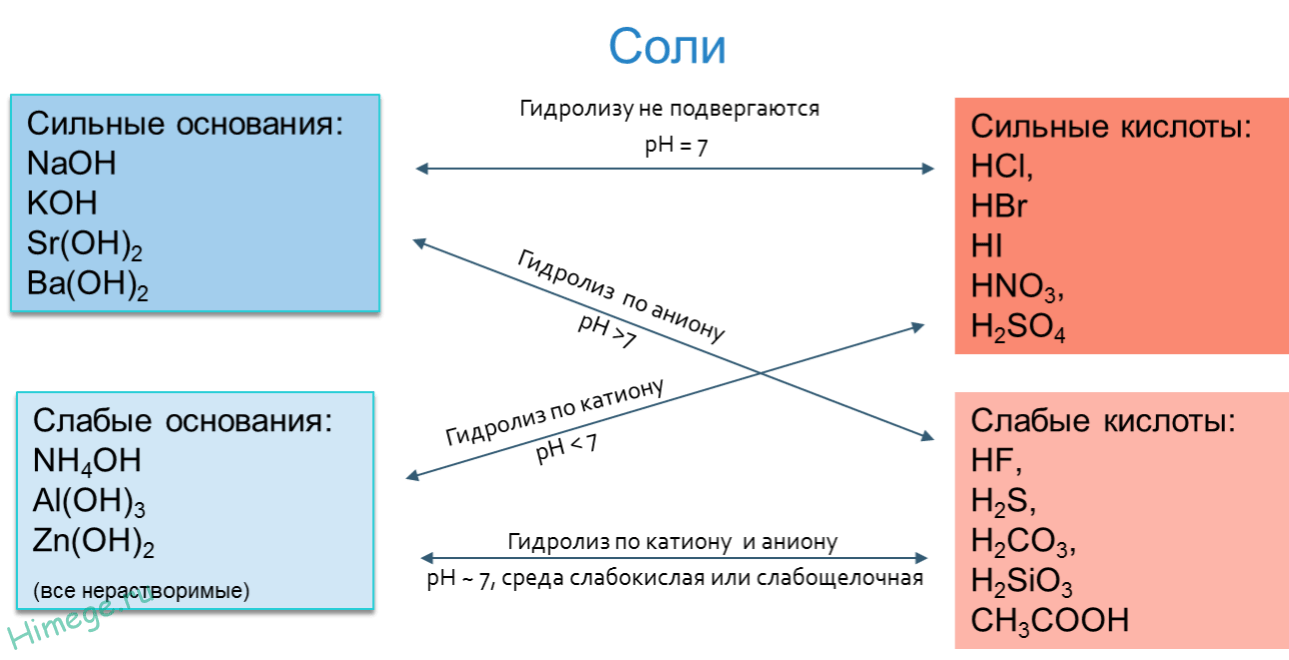
\includegraphics[width = 0.7\textwidth]{TeX/Pictures/17_acidbase.png}
    \caption{Диссоциация кислот и оснований}
    \label{fig:acidbase}
\end{figure}

\subsubsection{Слабое основание + сильная кислота}

В случае, если соль образована слабым основанием и сильной кислотой, она обратимо отдает ион \ce{H+} молекулам воды -- гиддролиз идет по катиону.


\ce{NH4Cl <--> NH4+ + Cl-} -- слабое онование + сильная кислота

\ce{NH4+ + HOH <--> NH4OH + H+} -- выделяются катионы водорода => среда кислая.

\ce{Cl- + HOH} $\neq$  

Итого:

\ce{NH4Cl + H20 <--> NH4OH + HCl}

Гидролиз по катиону, среда кислая (pH<7).

Константу гидролиза можно определить  через ионное произведение воды и константу диссоциации соответствующего катиону основания:

$\displaystyle K_h = \frac{[\ce{NH4OH}][\ce{H+}]}{[\ce{NH4+}]} = \frac{[\ce{NH4OH}][\ce{H+}][\ce{OH-}]}{[\ce{NH4+}][\ce{OH-}]}=\frac{K_\omega}{K_b(\ce{NH4OH})}$

Чем слабее основание(больше $K_b$), тем больше $K_h =>$ сильнее гидролиз соли по катиону.

\subsubsection{Сильное основание + слабая кислота}

\ce{CH3COOK <--> CH3COO- + K+} 

\ce{K+ + HOH} $\neq$

\ce{CH3COO- + HOH <--> CH3COOH + OH-} -- выделяются гидроксид-ионы, среда щелочная.

Итого:

\ce{CH3COOK + H2O <--> CH3COOK + KOH}

Гидролиз по аниону, среда щелочная, (pH>7),

Константу гидролиза по аниону также можно выразить через ионное произведение ыодф и константу диссоциации соответствующей аниону кислоты:

$\displaystyle K_h = \frac{[\ce{CH3COOH}][\ce{OH-}]}{[\ce{CH3COO-}]} = \frac{[\ce{CH3COOH}][\ce{H+}][\ce{OH-}]}{[\ce{CH3COO}][\ce{H+}]}=\frac{K_\omega}{K_a(\ce{CH3COOH})}$

Чем слабее кислота (чем меньше $K_a$, тем больше $K_h =>$ сильнее гидролиз соли по аниону)
\subsubsection{Слабое основание + слабая кислота}

\ce{CH3COONH3 <--> CH3COO- + NH4+}

\ce{CH3COO- + HOH <--> CH3COOH + OH-} -- выделяются гидроксид-ионы.

\ce{NH4Cl <--> NH4+ + Cl-}

\ce{NH4+ + HOH <--> NH4OH + H+} -- выделяются катионы водорода.

Итого:

\ce{CH3COONH4 + H2O <--> CH3COOH + NH4OH}

Гидролиз и по аниону и по катиону, среда нейтральная (pH=7).

\subsubsection{Сильное основание + сильная кислота}

\ce{Na2SO4 <--> 2Na+ + SO4^{2-}}

\ce{Na+ + HOH} $\neq$

\ce{So4^{2-} + HOH} $\neq$

Гидролиз не идет, среда нейтральная (pH=7).
 
 \subsection{Буферные растворы}
 
\begin{wrapfigure}[17]{r}{0.4\textwidth}
  \begin{center}
    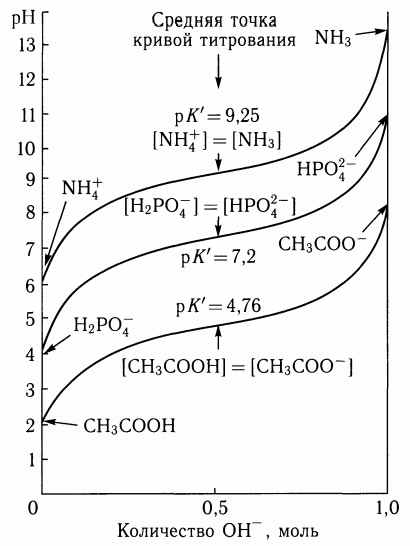
\includegraphics[width=0.38\textwidth]{TeX/Pictures/17_bufcurve.png}
  \end{center}
  \caption{Кривые титрования слабых кислот (\ce{CH3COOH, H2PO4-, NH+}) щелочью}
\end{wrapfigure}
 
 Рассмотрим кривые титрования растворо слабых кислот щелочью (зависимость pH раствора от количества добавленной щелочи). Видно, что в середине всех графиков есть пологий участок в диапазоне $pH = pK_a \pm 1$. То есть при добавлении даже значительного количества щелочи pH изменится слабо. Растворы с такими пропорциями называются буферными. 
 
 \Def{Кислотно-основные буферы} это смесь кислоты \ce{HA} и сопряженного ей основания \ce{A-} или  слабого основания \ce{B} и сопряженной ему кислоты \ce{BH+}
 
 Механизм действия буферной системы:
 
 Если к сопряженной паре \ce{HA}/\ce{A-} добавить сильную кислоту(\ce{H+}), то с ней прореагирует основание \ce{A-}:
 
 \ce{A-  + H+ -> HA}
 
 А если добавить щелочь, ее действие нейтрализуется кислотой \ce{HA}:
 
 \ce{HA + OH- -> A- + H2O}
 
 Кислотность раствора можно найти из концентраций [\ce{A-}] и [\ce{HA}]: $[\ce{H+}] = \frac{K_a[\ce{HA}]}{[\ce{A-}]}$ 
 
 \begin{equation}
     \text{Уравнение Гендерсона-Хассельбаха: }  pH = pK_a + \lg\frac{[\ce{A-}]}{[\ce{HA}]} 
 \end{equation}
 
 

\subsection{Кислоты и основания по Льюису}

\Def{Основания Льюиса} – это доноры пары электронов (все анионы, аммиак и амины, вода, спирты, галогены).

\Def{Кислоты Льюиса} – это акцепторы пары электронов, т.е. соединения, имеющие вакантную орбиталь (ион водорода и катионы металлов: \ce{H+, Ag+, Na+, Fe^{2+}}; галогениды элементов второго и третьего периодов \ce{BF3, AlCl3, FeCl3, ZnCl2}; галогены; соединения олова и серы: \ce{SnCl4, SO3}).

\begin{equation}
\ce{BF3 + F- ->}[\ce{BF4}]    
\end{equation}


\begin{figure}[H]
    \centering
    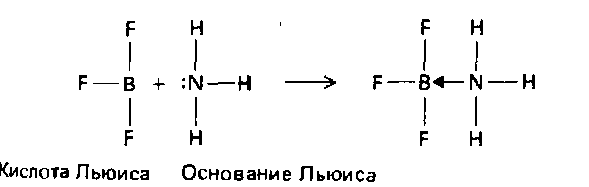
\includegraphics{TeX/TeX_Files/17_luis.png}
    \caption{Взаимодействие основания и кислоты Льюиса — образование связи по донорно-акцепторному механизму}
    \label{fig:luis}
\end{figure}

\newpage

\section{}

\newpage

\section{}

\newpage

\section{}

\newpage

\section{Положение неметаллов в Периодической системе. Типичные свойства и степени окисления неметаллов. Основные типы соединений, образуемых неметаллами.}

Неметаллические свойства элементов определяются способностью атомов ''принимать'' электроны, т.е. проявлять при взаимодействии с атомами других элементов окислительные свойства.

Неметаллы в таблице Менделеева находятся справа сверху над диагональю от бериллия к астату (см. рисунок \ref{fig:21.mendel})

\begin{figure}[H]
	\centering
	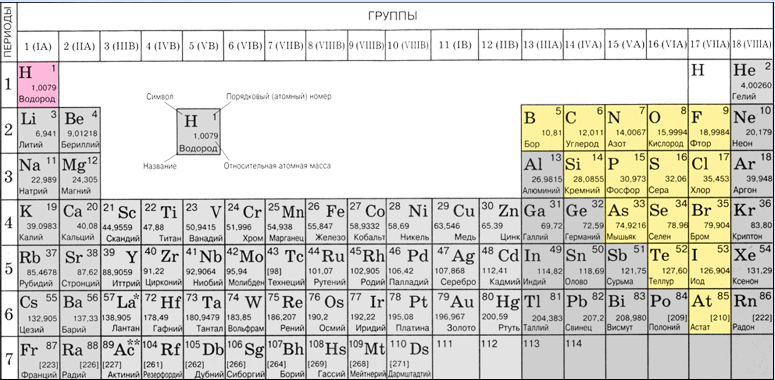
\includegraphics[width=0.7\linewidth]{21.mendel}
	\caption{Положение неметаллов в таблице Менделеева. Выделены цветом.}
	\label{fig:21.mendel}
\end{figure}

Практически все неметаллы имеют сравнительно малые радиусы и большое число электронов на внешнем энергетическом уровне от 4 до 7, для них характерны высокие значения электроотрицательности и преимущественно окислительные свойства.

\begin{figure}[H]
	\centering
	
\includegraphics[width=0.7\linewidth]{21.electric}
	\caption{Ряд электроотрицательности (фрагмент)}
	\label{fig:21.electric}
\end{figure}


Галогены, азот, кислород, водород как простые вещества существуют в виде двухатомных молекул (\ce{F2, Cl2, Br2, I2, N2, O2, H2}). Остальные неметаллы могут существовать при нормальных условиях, как в кристаллическом состоянии, так и в аморфном состоянии. Неметаллы в отличие от металлов плохо проводят теплоту и электрический ток.

Для неметаллов также характерно проявление \textbf{аллотропии} --- существования элемента в форме различных простых веществ, различающихся либо строением и составом молекул (кислород и озон), либо способом упаковки (алмаз и графит). Пример аллотропных модификаций приведен на примере фосфора на рисунке \ref{fig:21.p}.

\begin{figure}[H]
	\centering
	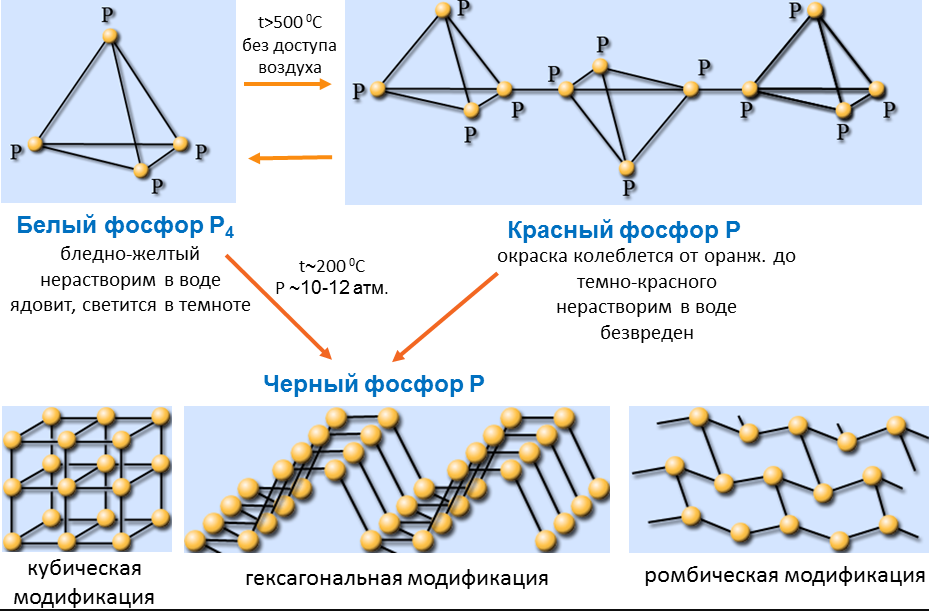
\includegraphics[width=0.7\linewidth]{21.p}
	\caption{Аллотропные модификации фосфора}
	\label{fig:21.p}
\end{figure}

\subsection{Химические свойства неметаллов}

Наиболее характерными степенями окисления для неметаллов являются отрицательные степени окисления, т.к/т.е. в большинстве реакций они выступают в роли окислителей. Иногда, при взаимодействии с более электроотрицательными неметаллами, например, они могут проявлять восстановительные свойства и принимать положительные степени окисления.

Если неметалл может образовывать соединения с разными степенями окисления, то свойства соединений будут зависеть от степени окисления элемента. С увеличением степени окисления кислотные свойства соединений увеличиваются.

\begin{enumerate}
	\item Для неметаллов характерны реакции с металлами, при это они проявляют окислительные свойства и в образующихся бинарных соединениях проявляют отрицательную степень окисления:
	
	\begin{align}
		\ce{Ca + H2 -> CaH2}\\
		\ce{2 Ca + O2 -> 2CaO}
 	\end{align}

	\item Неметаллы могут также взаимодействовать и с другими неметаллами, при этом более электроотрицательный металл играет роль окислителя, менее электроотрицательный --- роль восстановителя:
	
	\begin{align}
		\ce{S + 3 F2 -> SF6} \\
		\ce{H2 + Cl2 -> 2HCl}
	\end{align}

	При реакции с водородом неметаллы образуют летучие соединения (в обычных условиях это газы). Их водные растворы могут проявлять как основные (NH3, PH3), так и кислотные (\ce{HCl, HF}) свойства. В периоде с увеличением заряда ядра кислотные свойства водородных соединений неметаллов в водных растворах увеличиваются.

	При реакции с кислородом неметаллы образуют кислотные оксиды, проявляющие кислотные свойства. Они увеличиваются в периоде и уменьшаются в группе.

	При этому наиболее типичные неметаллы --- галогены (\ce{F}, \ce{Cl}, \ce{Br}, \ce{I}) --- с кислородом не реагируют (строго говоря, соединения попросту являются неустойчивыми), однако их можно получить косвенным путем, например \ce{F2O} можно получить при пропускании фтора через 2\%-ый водный раствор \ce{NaOH}:
	
	\begin{equation}
		\ce{2F2 + 2NaOH -> F2O + 2NaF + H2O}
	\end{equation}

	Однако, как и было сказано, подобная реакция очень капризна к условиям и при увеличении концентрации \ce{NaOH} выход \ce{F2O} резко уменьшится из-за протекания побочной реакции:
	
	\begin{equation}
		\ce{F2O + 2NaOH -> O2 + 2NaF + H2O}
	\end{equation}
\end{enumerate}

\newpage

\section{}

\newpage

\section{}

\newpage

\section{}

\newpage

\section{}

\newpage

\section{Понятие комплексного соединения. Координационная теория Вернера. Типы центральных атомов и лигандов. Геометрическое строение, координационные числа и изомерия комплексов.}

\textbf{Комплексные (координационные) соединения} --- соединения, которые образуются в результате присоединения к некоторому атому или иону (его называют \textbf{комплексообразователем}) нейтральных молекул или других ионов, которые называются \textbf{лигандами}.

\end{document}